\section{CI/CD workflow and release management}

\acrfull{ci} and \acrlong{cd} are the two key parts of the software development process that help developers deliver high-quality software. \acrlong{ci} (\acrshort{ci}) is the practice of automating the integration of code changes into a version control repository \cite{atlassianContinuousIntegrationVs}, encouraging developers to merge their changes to the main branch as often as possible. \acrshort{ci} establishes an automated method for building, packaging and testing the software. The main benefit of this approach is to avoid major integration challenges when releasing a version by continuously integrating more minor changes during the development instead of doing all the integration on the release day.

Whereas \acrlong{cd} (\acrshort{cd}) is an extension of continuous integration, where the code changes are automatically deployed to the production environment after the build and test stage. \acrshort{cd} aims to simplify the deployment as much as possible, making it a routine process that can be performed as many times as needed, even multiple times during a day \cite{WhatCICD}. Note that there is a distinction between Continuous Delivery and Continuous Deployment where the former requires human intervention to deploy changes to production, and the latter is fully automated without any manual steps.

\begin{figure}[ht]
  \centering
  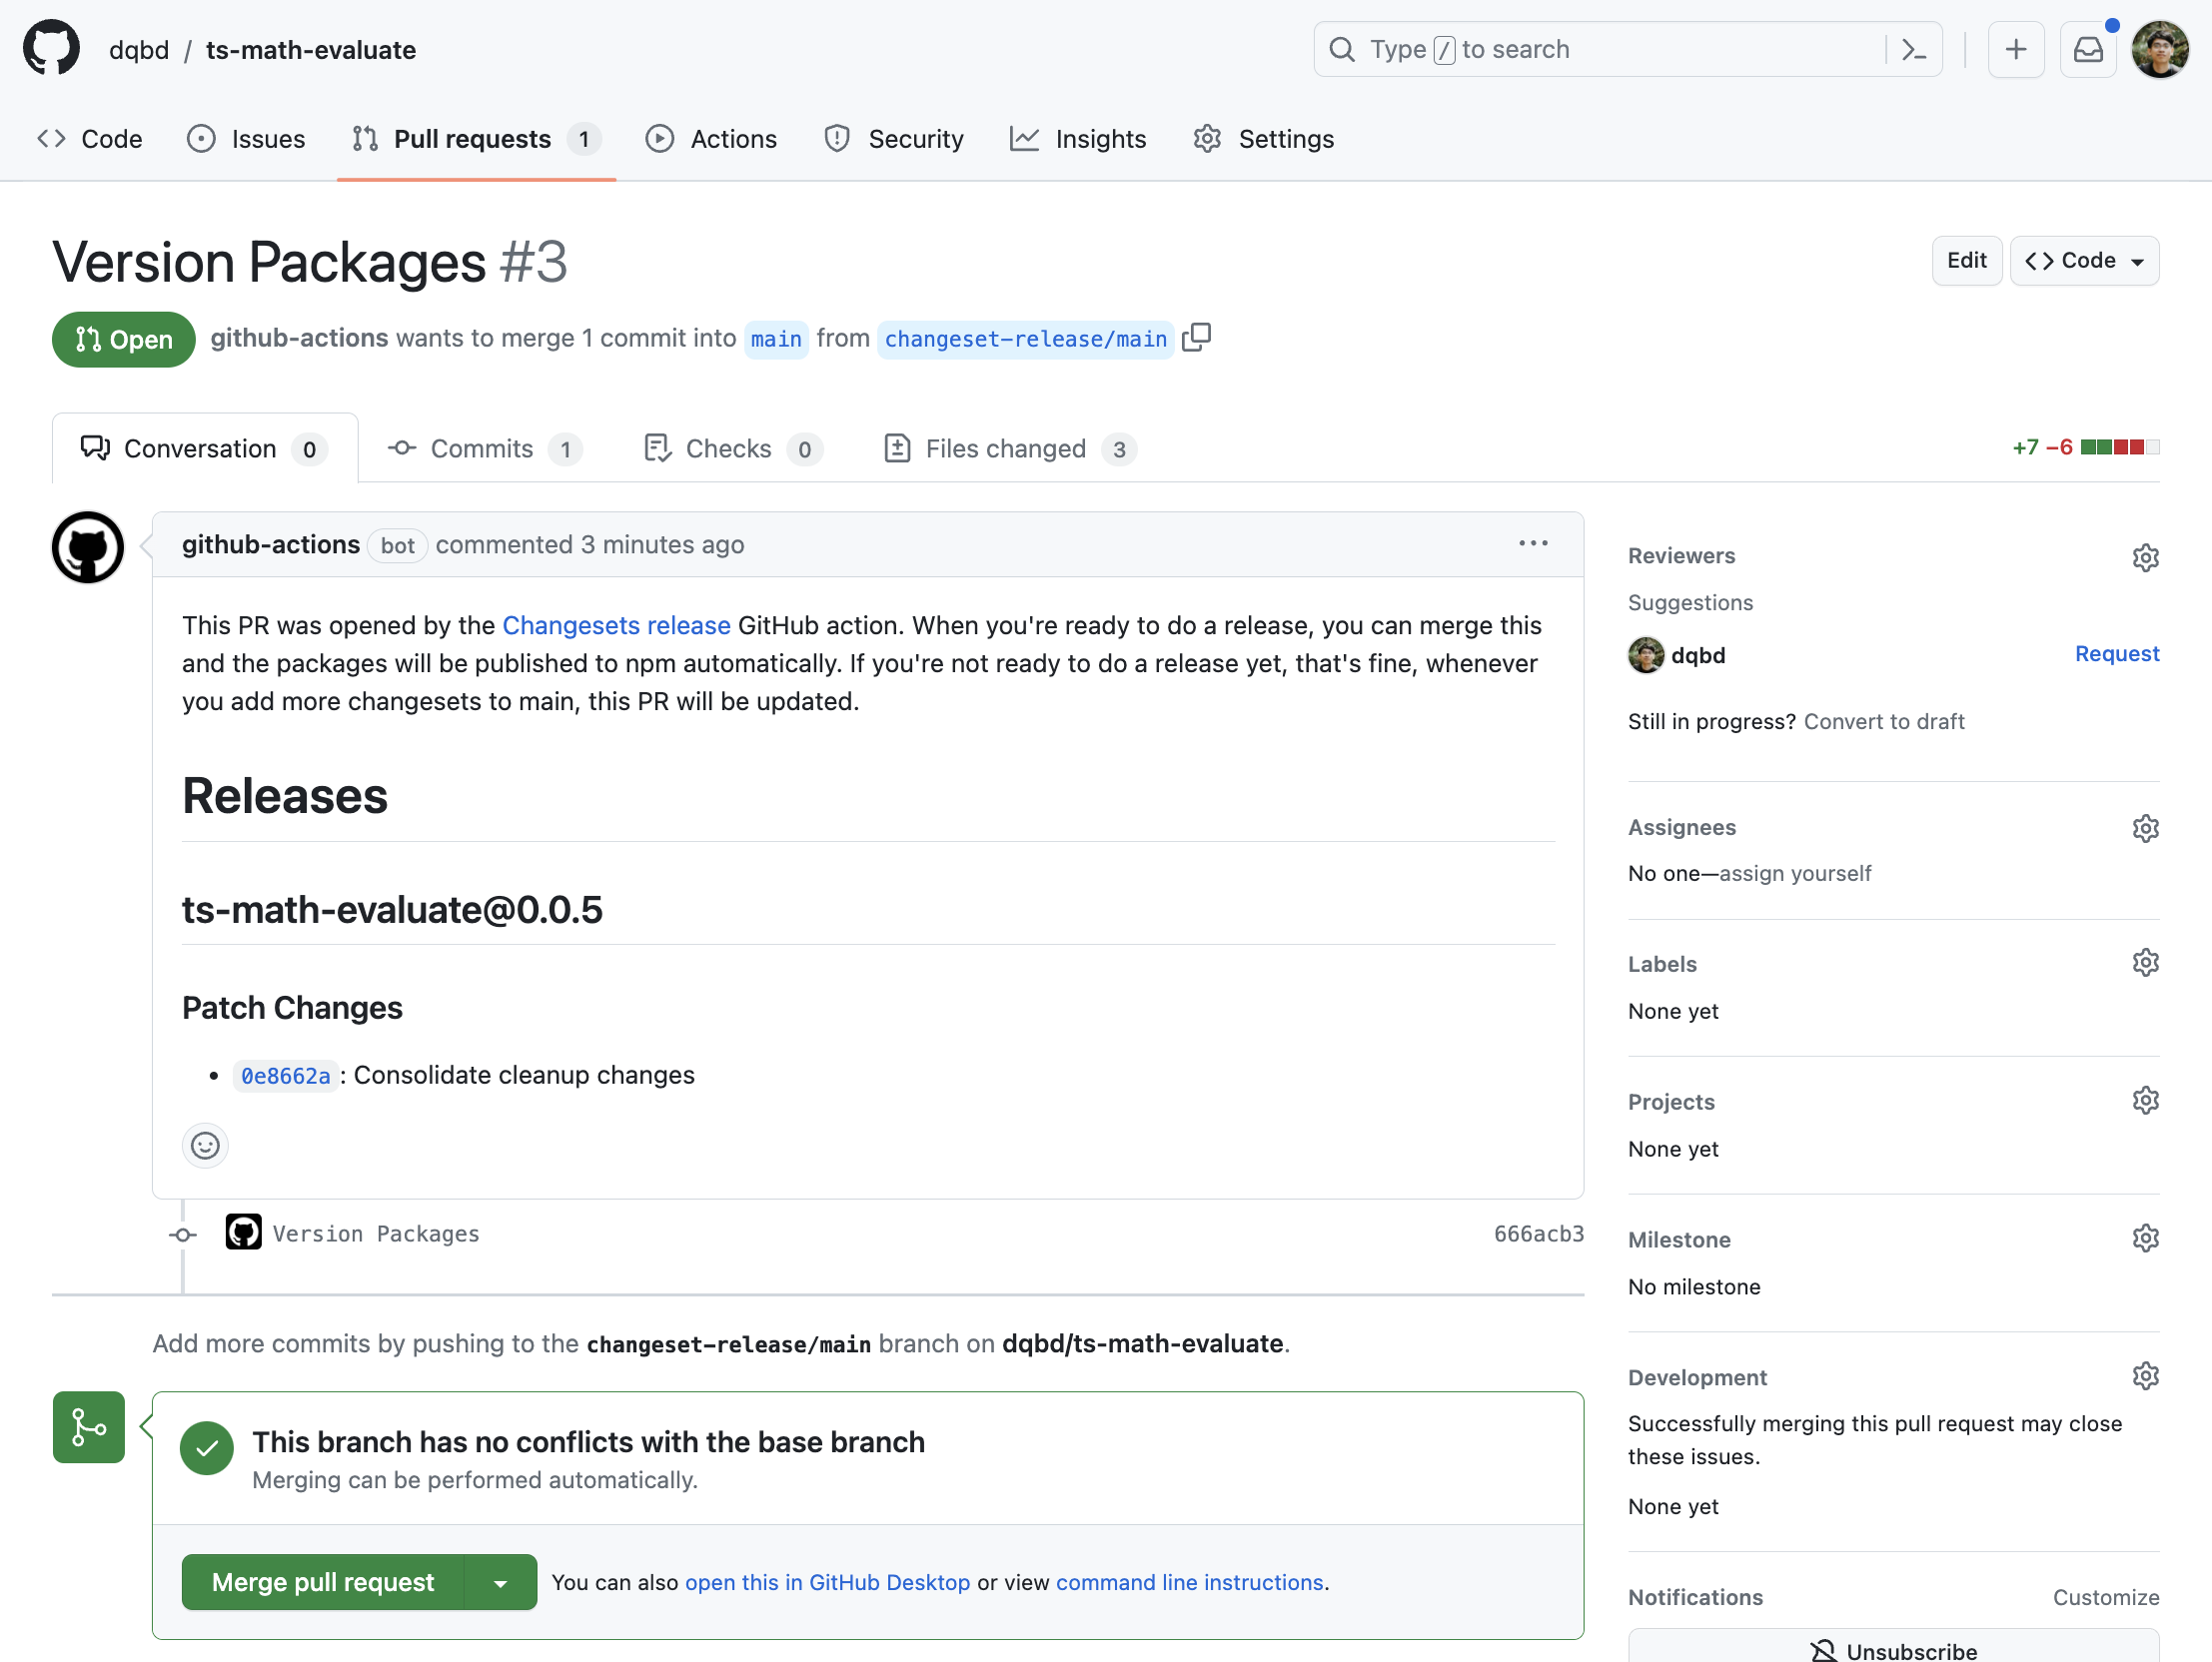
\includegraphics[width=\textwidth]{text/testing/changesets-pull-request.png}
  \caption{Pull request created by the Changesets Github Action}
  \label{fig:changesets-pull-request}
\end{figure}

Both Continuous Integration and Continuous Delivery are set up in the implementation part of the thesis. The core of the \acrshort{ci}/\acrshort{cd} setup is the Github Action platform. The GitHub Actions platform allows developers to automate the build, test, and deployment pipeline within an existing GitHub repository \cite{UnderstandingGitHubActions}. The main components of GitHub Actions include workflows, jobs and actions defined using YAML files saved in the \code{.github/workflows}. This project uses two workflows, one for running unit and integration tests and a second one for performing \acrfull{cd} to the \acrshort{npm} registry.

The first workflow, found in \code{.github/workflows/main.yml}, runs both \code{yarn run test} and \code{yarn run build} after every push to the repository event, regardless of branch or reference. The second workflow, found in \code{.github/workflows/publish.yml}, is responsible for handling releases to the \acrshort{npm} registry using Changesets \cite{ChangesetsChangesets2023}. Changesets allow developers to keep track of the release history of a package and automate both versioning and release note generation.

The Changesets tool works by separating versioning into two stages: adding a changeset, describing the changes made in a commit or a branch, and combining created changesets with a version incrementing.


Creation of a changeset is done by running the \code{yarn changeset} command, which will ask the developer to provide the appropriate version bump type (either MAJOR, MINOR or PATCH, following the Semver versioning) and a message describing the changes. The changeset will be saved as a Markdown file with a unique identifier in the \code{.changesets} folder. The file will be committed to the Git repository. These changesets are preserved in the repository until the release is ready to be published by merging the changesets into the \code{main} branch.

After a push event to the \code{main} branch occurs, the release process, defined as a GitHub Actions job, is launched. The release process itself works by running the \code{yarn changeset publish} command and works as such; When new changesets are found in the \code{main} branch, Changesets will, as seen in Figure \ref{fig:changesets-pull-request}, automatically create a new pull request, which will perform all of the key steps for releasing a package: incrementing the version, updating the \code{CHANGELOG.md} file and removing the accumulated changelogs. When the pull request is merged, Changesets will automatically publish the new version to the \acrshort{npm} registry, using the granular access token provided as a secret variable for \acrshort{ci}, and create an appropriate Git tag for the release. The final package is published to the \acrshort{npm} registry under the name \code{ts-math-evaluate} \cite{Tsmathevaluate2023}. 